%! Tex program = xelatex
\documentclass[]{article}
\usepackage[utf8]{inputenc}
\usepackage{ctex}
\usepackage{textcomp}
\usepackage{lmodern}
\usepackage[margin=1in]{geometry}
\usepackage{graphicx, color}
\usepackage{mathtools}
\usepackage{listings}
\usepackage{hyperref}

\usepackage{tikz}
\usetikzlibrary{automata,positioning}

\renewcommand{\epsilon}{\varepsilon}
\newcommand{\tikzname}{Ti\emph{k}Z}
\tikzset{shorten >=1pt, node distance=2cm, on grid, baseline={([yshift=-8pt] current bounding box.north)}}


\lstset{basicstyle=\small\ttfamily,breaklines=true}

\title{CS143 Spring 2022 -- Written Assignment 1}

\begin{document}
\begin{center}
% Change this:
\LARGE 龚开宸 \\
\LARGE 编译原理实验一
\end{center}

\begin{enumerate}
    \item 8进制数\, 状态转换图 \\
    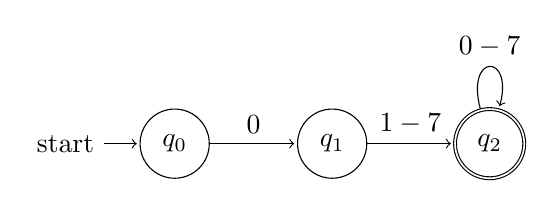
\begin{tikzpicture}[auto]
        \node[state,initial]   (q_0)                      {$q_0$};
        \node[state]           (q_1) [right of=q_0] {$q_1$};
        \node[state,accepting] (q_2) [right of=q_1] {$q_2$};
        \path[->]
            (q_0) edge [above]   node {$0$} (q_1)
            (q_1) edge [above]   node {$1- 7$} (q_2)
            (q_2) edge [loop above] node {$0-7$} (q_2); % 注意每一行都有分号
    \end{tikzpicture}

    \item 10进制\, 状态转换图 \\
        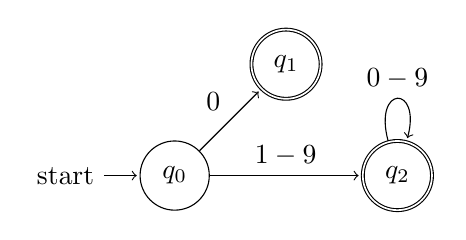
\begin{tikzpicture}[auto]
        \node[state, initial]   (q_0)                   {$q_0$};
        \node[state, accepting] (q_1) [above right of=q_0] {$q_1$}; % 第三个词有个 of
        \node[state, accepting] (q_2) [below right of=q_1] {$q_2$};
        \path[->]
            (q_0) edge  node {$0$} (q_1)
            (q_0) edge  node {$1-9$} (q_2)
            (q_2) edge[loop above]  node {$0-9$} (q_2);
    \end{tikzpicture}

    \item 16进制数\, 状态转换图 \\
    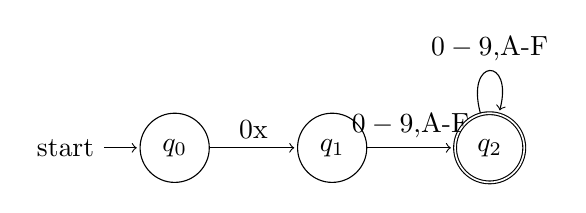
\begin{tikzpicture}[auto]
        \node[state,initial]   (q_0)                      {$q_0$};
        \node[state]           (q_1) [ right of=q_0] {$q_1$};
        \node[state,accepting] (q_2) [ right of=q_1] {$q_2$};
        \path[->]
            (q_0) edge    node {$0\text{x}$} (q_1)
            (q_1) edge    node {$0 - 9$,A-F} (q_2)
            (q_2) edge [loop above] node {$0 - 9$,A-F} (q_2); % 注意每一行都有分号
    \end{tikzpicture}

    \item Identifier\, 状态转换图 \\
    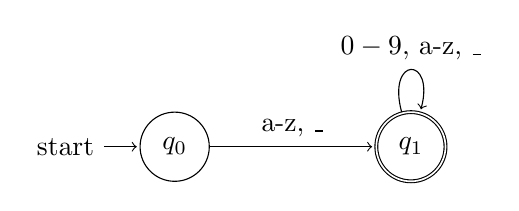
\begin{tikzpicture}[node distance=3cm,auto]
        \node[state,initial]   (q_0)                      {$q_0$};
        \node[state,accepting] (q_1) [ right of=q_0] {$q_1$};
        \path[->]
            (q_0) edge    node {a-z, \_} (q_1)
            (q_1) edge[loop above]    node {$0 - 9,$ a-z, \_} (q_1);
    \end{tikzpicture}


\item 关键字,  仅以 if 为例 \\
    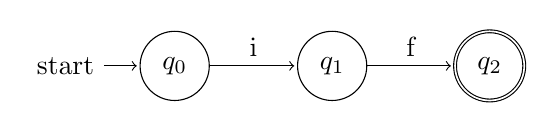
\begin{tikzpicture}[auto]
        \node[state,initial]   (q_0)                      {$q_0$};
        \node[state]           (q_1) [right of=q_0] {$q_1$};
        \node[state,accepting] (q_2) [right of=q_1] {$q_2$};
        \path[->]
            (q_0) edge [above]   node {i} (q_1)
            (q_1) edge [above]   node {f} (q_2);
    \end{tikzpicture}

\item 关键字,界符
    \begin{tikzpicture}[node distance=4cm,auto]
        \node[state,initial]   (q_0)                      {$q_0$};
        \node[state,accepting]  (q_1) [right of=q_0] {$q_1$};
        \path[->]
            (q_0) edge [above]   node {关键词,界符} (q_1);
    \end{tikzpicture}

\item write \LaTeX on neovim is a pleasure
    \begin{displaymath}
        \sum_{n=1}^{\infty} a_n z^n \quad
        \sum_{n=1}^{\infty} a_n z^n
    \end{displaymath}

\end{enumerate}
\newpage
\end{document}
